\selectlanguage{english}
\chapter{The CMS detector at LHC}
\label{Chapter2}
%SourceDoc tesi.tex

\section{The Large Hadron Collider}
Approved in the early '90s and started up in the 2008, the \textit{Large Hadron Collider} (LHC)  is currently the world's largest and most powerful particle accelerator. \\
Its main purpose is to help in testing the predictions of different theories of particle physics. \\
%, including the search of the Higgs boson and the dark matter. \\
LHC \cite{LHC},  situated at the CERN laboratories of Geneva, is a proton-proton (pp) collider built to work at the design center of mass energy of $\sqrt{s} = 14$ TeV, with a bunch crossing every 25 ns and a design luminosity of $10^{34}$ cm$^{-2}$ s$^{-1}$. It is  installed in the same circular underground tunnel occupied until the year 2000 by the Large Electron Positron
collider (LEP). The $pp$ collision are used, instead of the $e^+e^-$ one of LEP, to reduce the synchrotron radiation, in order to accelerate the particles up to a very large energy. It was preferred to a $p\bar{p}$ collider because it allows to reach higher rate of events. In fact the low anti-proton production efficiency ($10^5$ protons are needed to create an anti-proton) and larger time needed to accumulate them, would make almost impossible to reach the high design luminosity of the LHC. The luminosity $L$ is the parameter to quantify the performances of a collider, because the event rate $R_i$ of a given process $i$, defined as the number of events occurring per unit of time, can be written as:
\begin{equation}
R_i = \frac{dN_i}{dt}=L\cdot \sigma_i
\end{equation}
where $\sigma_i$ is the cross section of the process $i$. The luminosity depends only on the machine parameters. Assuming a small crossing angle between the
beams and Gaussian-shaped beam bunches, the luminosity $L$ can be written as:
\begin{equation}
L=\frac{fn_bN^2}{4\pi\sigma^2}
\end{equation}
where $f$ is the revolution frequency of particle bunches, $n_b$ is the number of bunches rotating in the accelerator, $N$ is the number of protons in the two colliding bunches and $\sigma$ is the RMS of beam profile distributions in the plane orthogonal to the beam direction. \\
%LHC is a 26.7 km ring of superconducting magnets with a number of accelerating structures to boost the energy of the particles along the way. It is not a perfect circle: it is made of eight arcs and eight insertions. The arcs are long 106.9m with a curvature of 2.84km containing 1232 superconductive dipoles. The LHC dipoles use Niobium-Titanium (NbTi) cables at a temperature of 1.9K, pumping superfluid helium into the magnet system, where they become superconducting; a current of 11850A flows in the dipoles to create the high magnetic field of 8.33 T required to bend the beams around the ring. The insertions instead consist of a long straight section of 528m plus two (one at each end) transition regions. They contains the radiofrequency cavities to increase beam energy (0.5 MeV per period): there are eight cavities per beam, each delivering 2MV (an accelerating field of 5MV/m) at 400MHz operating at 4.5K. Particular kind of insertion are quadrupoles, special magnets used to focus the beam down to the smallest possible size at the collision points: there 392 quadrupoles in LHC. The two beams will run in two contiguous pipes with vacuum inside, separated by 19.4 cm, that will be unified in proximity of the interactions points, where the experiments will be placed. Because of the high luminosity of the LHC, large thermal power will be generated near the pipes due to the synchrotron radiation, making necessary the presence of a suitable cooling system. For this reason also the pipes will be in contact with superfluid Helium at 1.9 K. \\
In the LHC design, 1232 main dipole magnets (made of niobium-titanium super-conductor chilled with superfluid Helium at 1.9 K) generating a magnetic field up to 8.3 T, will be used to steer the particles into curvilinear trajectories. The two beams will run in two contiguous pipes with vacuum inside, separated by 19.4 cm, that will be unified in proximity of the interactions points, where the experiments will be placed. Because of the high luminosity of the LHC, large thermal power will be generated near the pipes due to the synchrotron radiation, making necessary the presence of a suitable cooling system. For this reason also the pipes will be in contact with superfluid Helium at 1.9 K. \\
In \figurename~\ref{Cern-Accelerator-Complex}  is shown the complete scheme of the accelerator chain of the LHC: the proton beam is created by using an electric field to pull the electrons from hydrogen atoms and start the acceleration. Protons are injected into the PS Booster (PSB) at an  energy of 50 MeV from Linac2 (Linear Accelerator 2). The booster comprises four superposed rings: this is because at low energy intensity, the quality of the beams suffers from the repulsive forces between particles. By splitting up the injected beam this effect gets reduced. Once the beam reaches the energy of 1.4 GeV it is extracted and injected into Proton Synchrotron (PS). With a circumference of 628 m, the PS accelerates the beams up to 26 GeV when they are extracted and sent to the Super Proton Synchrotron (SPS). Built in the '70, the SPS has a length of 7 km. The beam is injected at 26 GeV, ramped up to 450 GeV and extracted to the LHC. \\%At the SPS, the boson W and Z were discovered and this led Rubbia and Simon van der Meer to win the Nobel prize. \\
\begin{figure}[htbp]
\centering
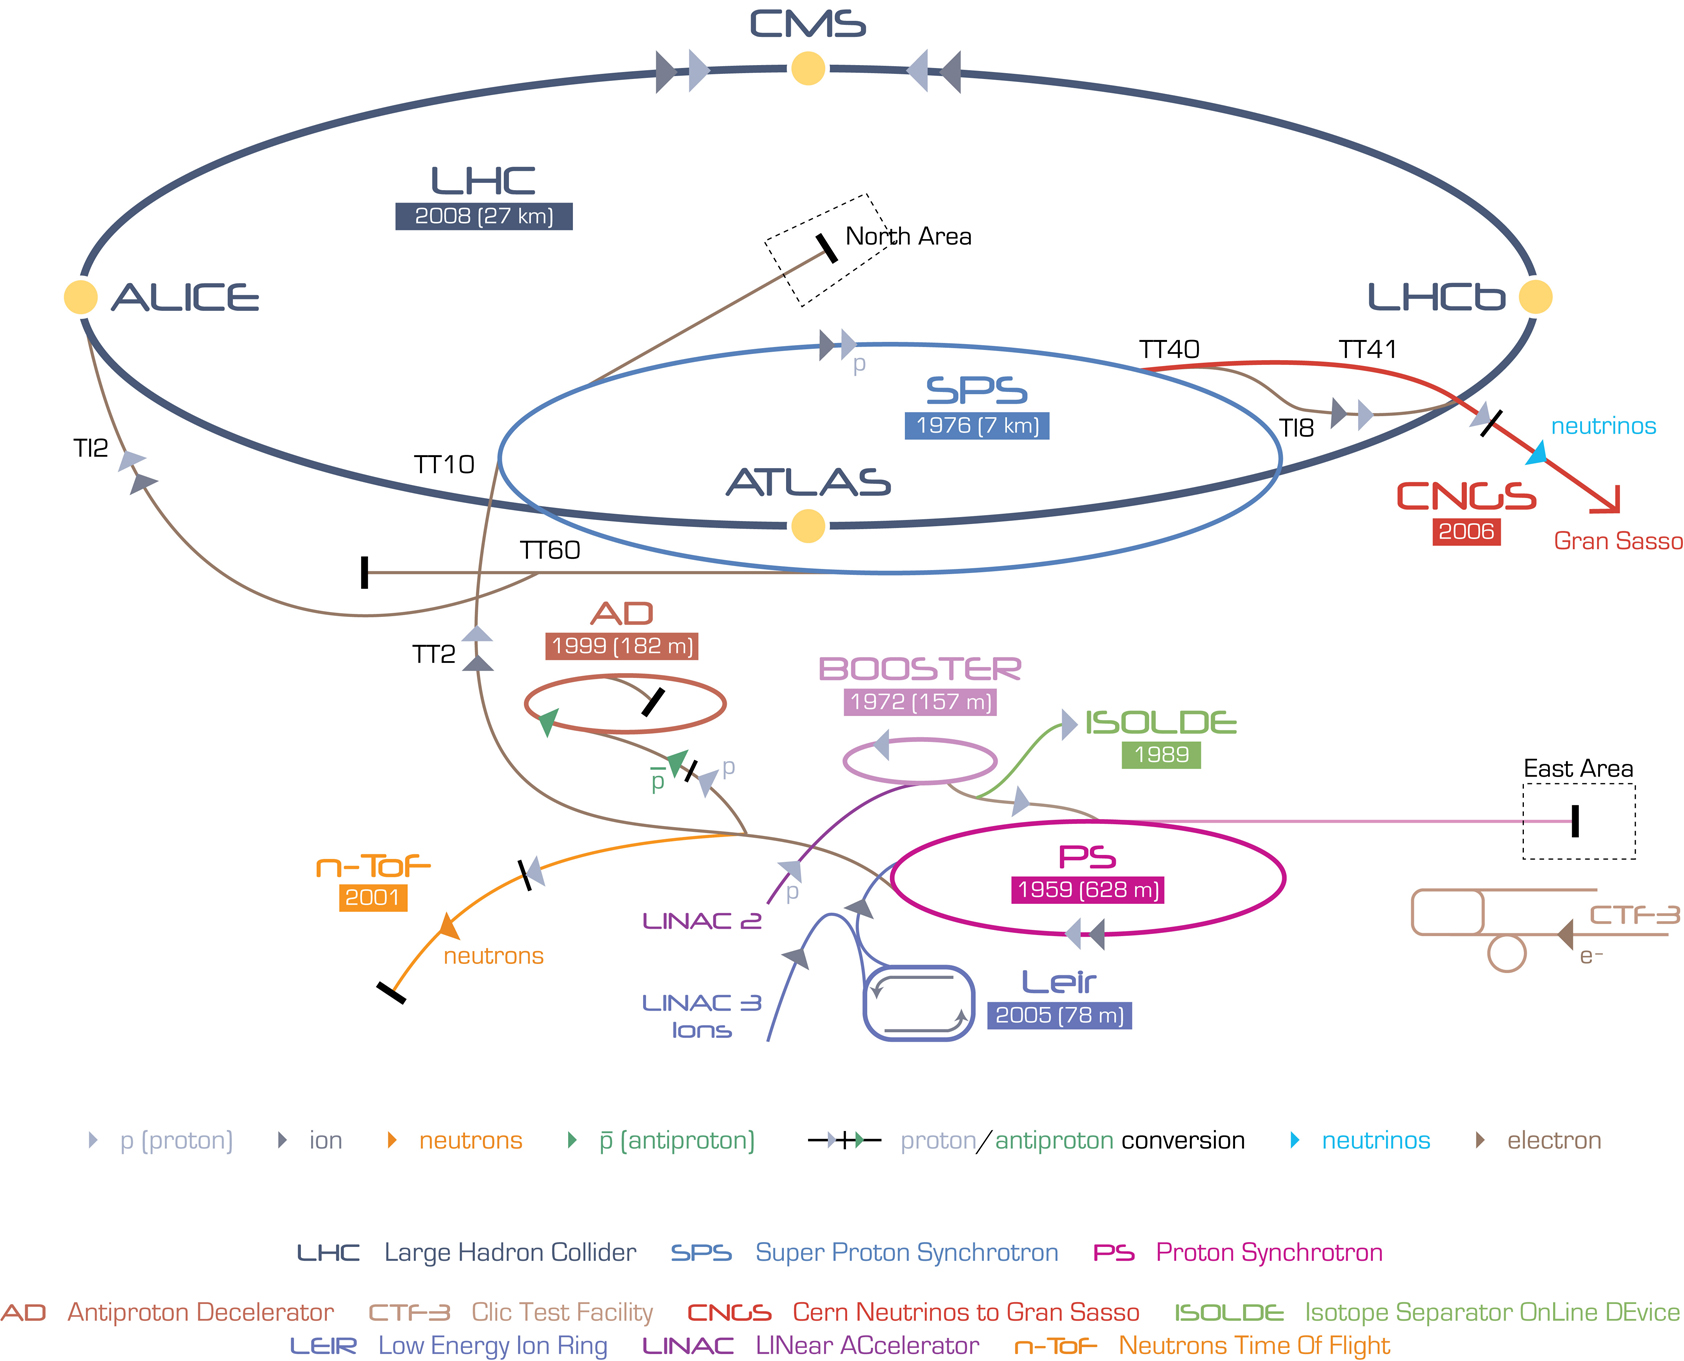
\includegraphics[width=0.65\textwidth]{Images/Cern-Accelerator-Complex}
\caption{Accelerator scheme at CERN.}
\label{Cern-Accelerator-Complex}
\end{figure}
Once the energy-working point is reached, the beams are made to collide at four locations around the LHC, corresponding to the position of four particles detectors: ALICE (\emph{A Large Ion Collider Experiment}), ATLAS (\emph{A Toroidal LHC ApparatuS}), CMS (\emph{Compact Muon Solenoid}) and LHCb (\emph{Large Hadron Collider beauty}). In addition to these, there are other three experiment installed at the LHC: TOTEM (\textit{TOTal Elastic and diffractive cross section Measurement}) installed close to CMS, MoEDAL (\textit{Monopole and Exotics Detector at the LHC}) close to LHCb and LHCf (\textit{Large Hadron Collider forward}) near ATLAS. \\
The beams at LHC have a bunch structure as a direct consequence of the radio frequency acceleration scheme. Protons can only be accelerated when the RF field has the correct orientation when particles pass through an accelerating cavity. Under nominal operating conditions, each proton beam has 2808 bunches, with each bunch containing about $10^{11}$ protons. The bunch size is not constant around the ring getting squeezed as much as possibile around the interaction points in order to increase the probability of collision. They measure a few centimetres long and a millimetre wide when they are far from a collision point; as the bunches approach  the collision points, they are squeezed to about $20\ \mu m$. LHC uses a bunch spacing of 25 ns (or 7.5 m) corresponding to a frequency of 40 MHz. \\
In \tablename~\ref{LHC_parameteres} are reported the designed LHC parameters and the ones reached at the end of RunII in 2018.
\begin{table}[htbp]	
	\begin{center}
		\begin{tabular}{p{6cm}*{3}{c}}
			\hline   &  & Design & 2018  \\
			\hline
			\hline
			\bfseries Centre of mass energy & \emph{E} & 14 TeV & 13 TeV \\
			\hline
			\bfseries Luminosity & \emph{L} & 10$^{34}$ cm$^{-2}$s$^{-1}$ & --- \\
			\hline
			\bfseries Time spacing &  & 25 ns & 25 ns\\
			\hline
			\bfseries Num. of bunches& \emph{k$_{B}$} & 2808 & ---\\
			\hline
			\bfseries Num. protons per bunch & \emph{N$_{p}$} & 1.15$\times$10$^{11}$ & ---\\
			\hline
			\hline
		\end{tabular}
	\end{center}
	\caption{LHC parameters}
	\label{LHC_parameteres}
\end{table}


\section{The Compact Muon Solenoid}\label{sec:cms}
The Compact Muon Solenoid (CMS) is one of the general purpose experiments which takes data at the LHC. Its physics goals range from the search for the Higgs boson to the searches for physics beyond the Standard Model, to the precision measurements of already known particles and phenomena \cite{CMS_Detector}. \\
The overall layout of CMS is shown in \figurename~\ref{CMS_Layout}. The inner tracker and the two calorimeters of CMS are located inside a $13\,$m-long, $5.9 \,$m inner diameter, $3.8\, $T superconducting solenoid. In order to achieve good momentum resolution within a compact spectrometer  without making stringent demands on muon-chamber resolution and alignment, a high magnetic field was chosen. The return field is large enough to saturate $1.5 \,$m of iron, allowing four muon stations to be integrated to ensure robustness and full geometric coverage. The central part of CMS is called \emph{barrel} while the two edges of the detector are denoted as \emph{endcaps}.
\begin{figure}[htbp]
\centering
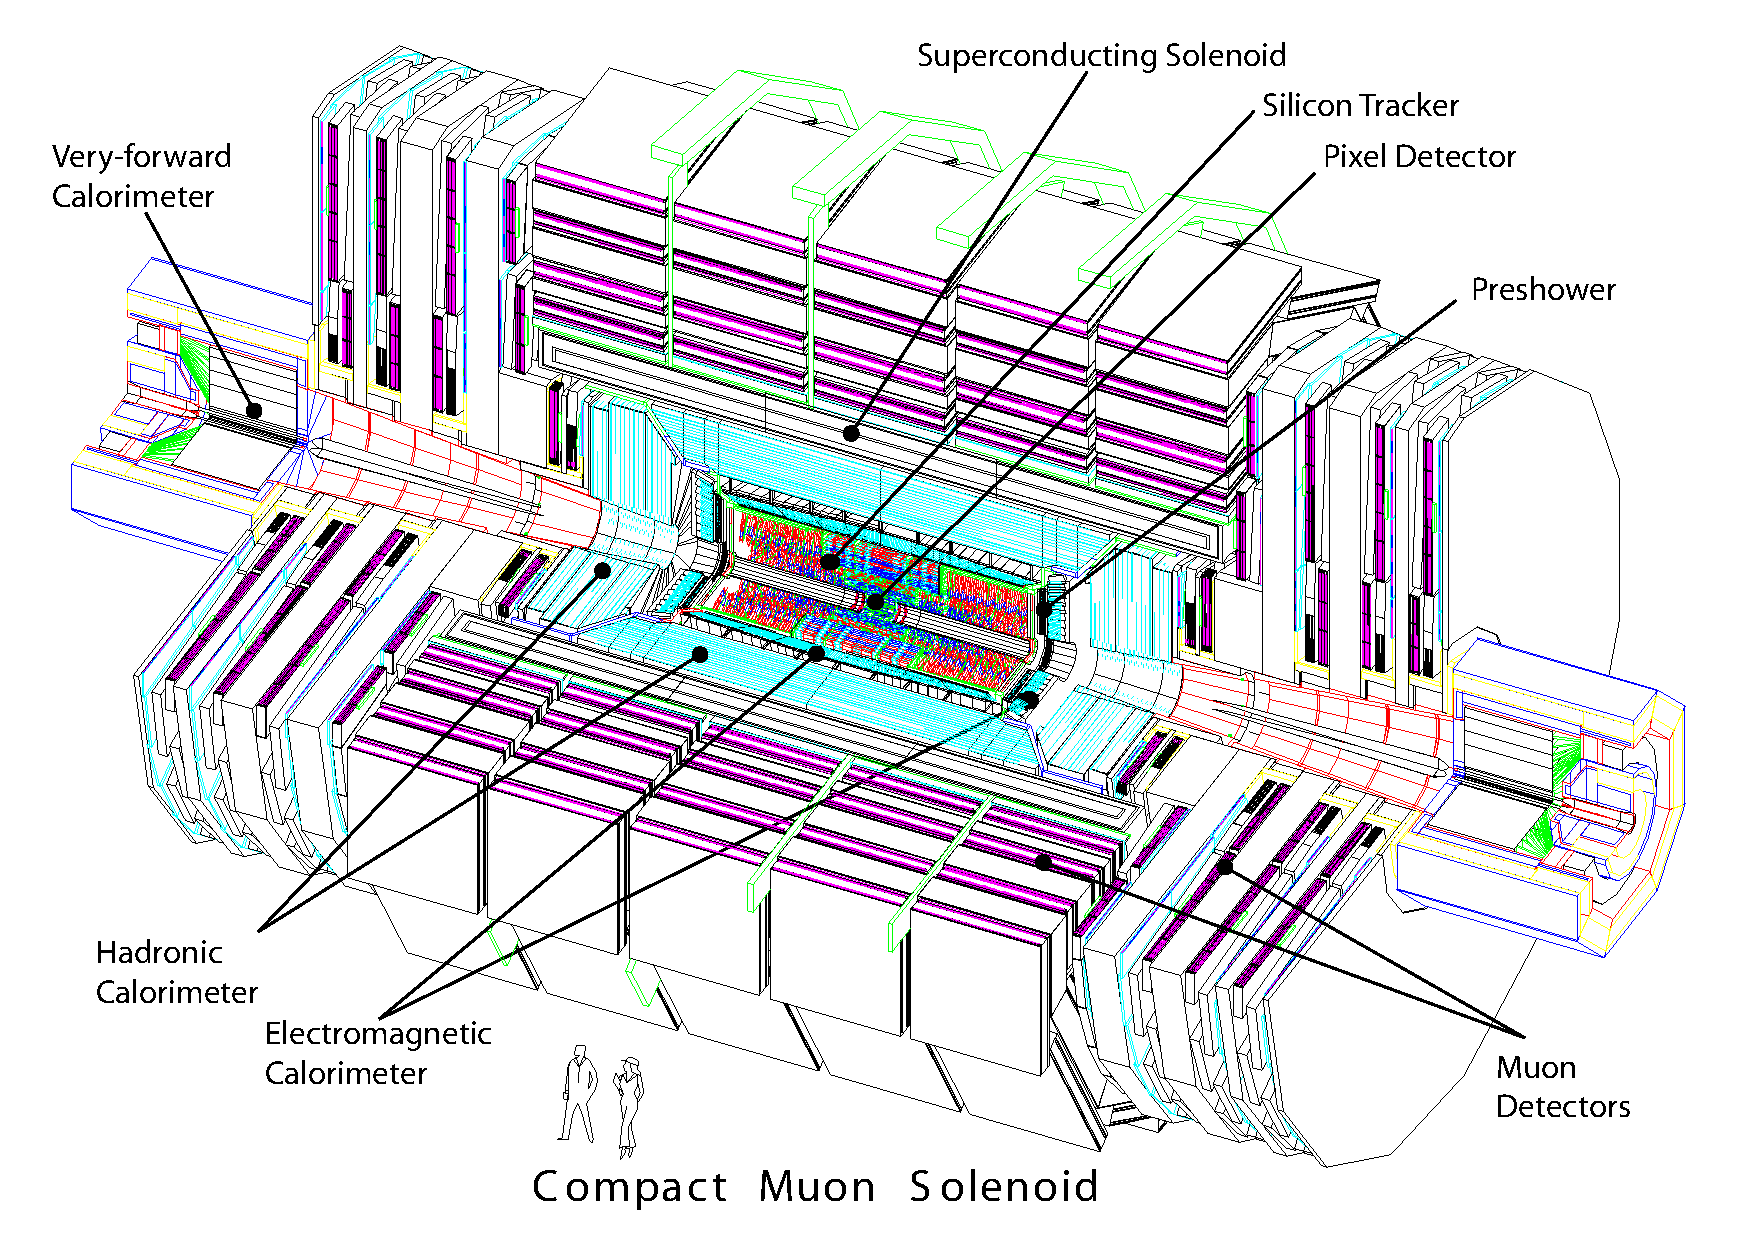
\includegraphics[width=0.7\textwidth]{Images/CMS_Layout.pdf}
\caption{CMS detector overview.}
\label{CMS_Layout}
\end{figure}
The tracking volume is given by a cylinder of length $5.8 \,$m and diameter $2.6 \,$m. In order to deal with high track multiplicities, CMS employs $10$ layers of silicon microstrip detectors, which provide the required granularity and precision. In addition, $3$ layers of silicon pixel detectors are placed close to the interaction region to improve the measurement of the impact parameter of charged-particle tracks, as well as the position of secondary vertexes. The electromagnetic calorimeter (ECAL) uses lead tungstate ($\mathrm{PbWO_4}$) crystals with coverage in pseudorapidity up to $|\eta| < 3.0$.  A preshower system is installed in front of the edges of ECAL for $\pi^0$ rejection.

%In the following, the CMS sub-detectors are described from the innermost region  (the closest to the interaction point) to the outermost region. The chapter ends with a description of the trigger and data acquisition systems.

\subsubsection{Coordinate Conventions}
The coordinate system adopted by CMS has the origin centered at the nominal collision point inside the experiment,  the $y$-axis pointing vertically upward, and the $x$-axis pointing radially inward toward the center of the LHC. Thus, the z-axis points along the beam direction toward the Jura mountains from LHC Point 5. 
\begin{comment}
Figure \ref{fig:coord} shows the coordinate system in CMS.
%\begin{sidewaysfigure}[htp]
\begin{figure}[h!]
 \centering
 %\includegraphics[width=13cm]{cms/img/cms_theDetector.png}
% \includegraphics[width=0.45\textwidth]{cms/img/coord.pdf}
 \caption{Coordinate system in CMS  \cite{Marcastel:1621583}.}
\label{fig:coord}
%\end{sidewaysfigure}
\end{figure}
\end{comment}
The azimuthal angle $\phi$ is measured from the $x$-axis in the $x$-$y$ plane. The polar angle $\theta$ is measured from the $z$-axis. Pseudorapidity is defined as 
\begin{equation}
\eta = -\ln \tan (\theta / 2)
\end{equation}
The value $\eta=0$ corresponds to a direction perpendicular to the beamline, while the limit $\eta = \infty$ gives a direction parallel to the beamline. The momentum and energy measured transverse to the beam direction, denoted by $p_T$ and $E_T$, respectively, are computed  as follow:
\begin{equation}
p_T = p sin \theta
\end{equation}

\begin{equation}
E_T = E sin \theta
\end{equation}

Finally, particles which escape the detection leave an imbalance in the transverse plane which is quantified as missing transverse energy in the following way:

\begin{equation}
E_T^{miss} = - \sum_i p_T^i
\end{equation}

as the negative vectorial sum of the transverse momentum of all the visible particles in the event.




\subsection{The tracking system}
\label{sec:tracker}
The tracker \cite{Tracker_1, Tracker_2} , placed within the magnetic field, is the subdetector which is closer to the interaction point. It is dedicated to track and vertex finding. The silicon (Si) technology has been chosen for the whole tracker in order to provide good radiation hardness, high granularity and large hit redundancy to perform a good pattern recognition. The layout of the CMS tracker is shown in \figurename~\ref{tracking_system}. Close to the interaction vertex, in the barrel region, are 3 layers of hybrid pixel detectors at a radius (r) of about 4, 7 and 10 cm. The size of the pixel detector is $100-150$ m$^2$. In the barrel part, the Si microstrip detectors are placed at r between 20 and 110 cm. The forward region has 2 pixel and 9 microstrip layers in each of the two endcaps. In order to avoid excessively shallow track crossing angles, the Inner Barrel is shorter than the Outer Barrel, and there are additional three Inner Disks in the transition region between barrel and endcaps, on each side of the Inner Barrel. The total area of the Si detectors is around 200 m$^2$, providing a coverage up to $\eta = 2.5$. The material budget inside the active volume of the tracker increases from $0.4$ radiation length ($X_0$) at $\eta= 0$ to around $1$  $X_0$ at $|\eta|= 1.6$, before decreasing to $0.6$ $X_0$ at $|\eta|= 2.5$. \\
\begin{figure}[h!]
 \centering
 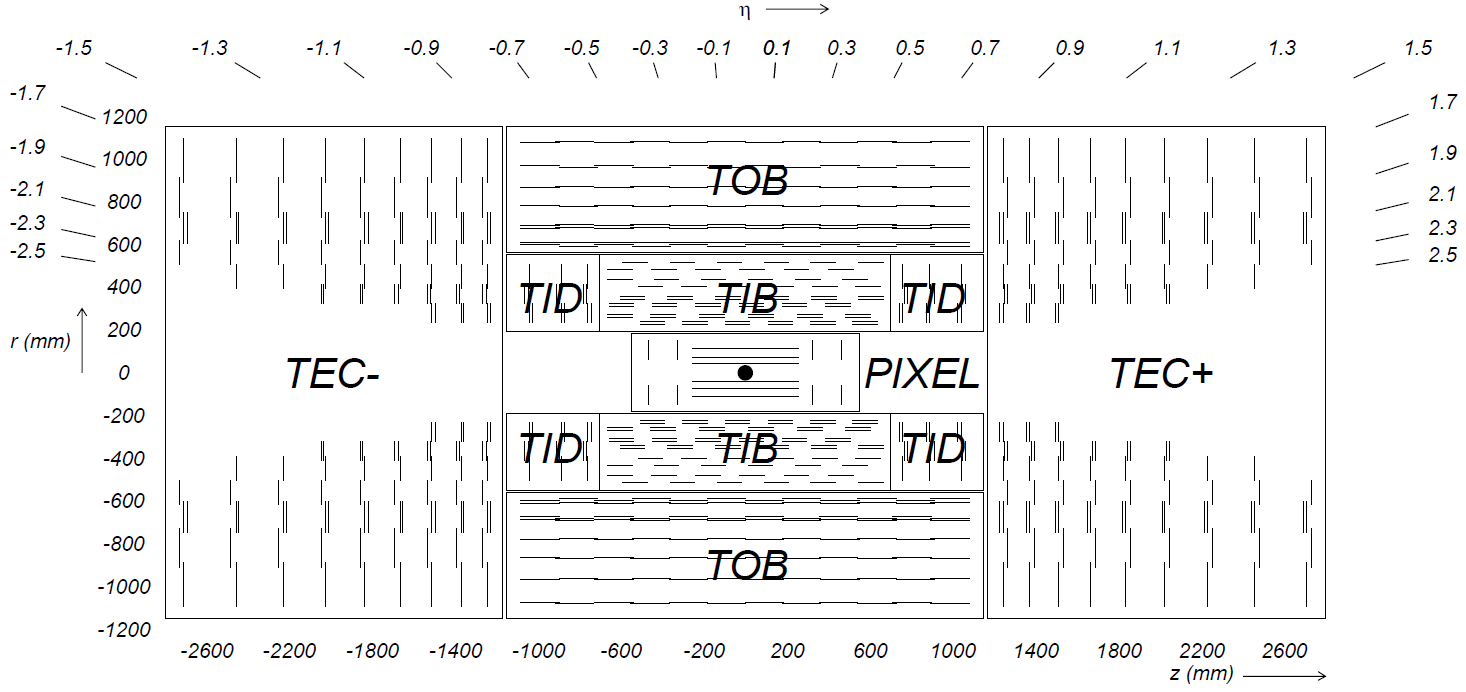
\includegraphics[width=0.9\textwidth]{Images/cmsTracker_TrackerLayout}
\caption{Schematic cross section through the CMS tracker in the $r-z$ plane: each line represents a detector module. Double lines indicate back-to-back modules which deliver stereo hits.}
\label{tracking_system}
\end{figure}
\begin{figure}[h!]
 \centering
 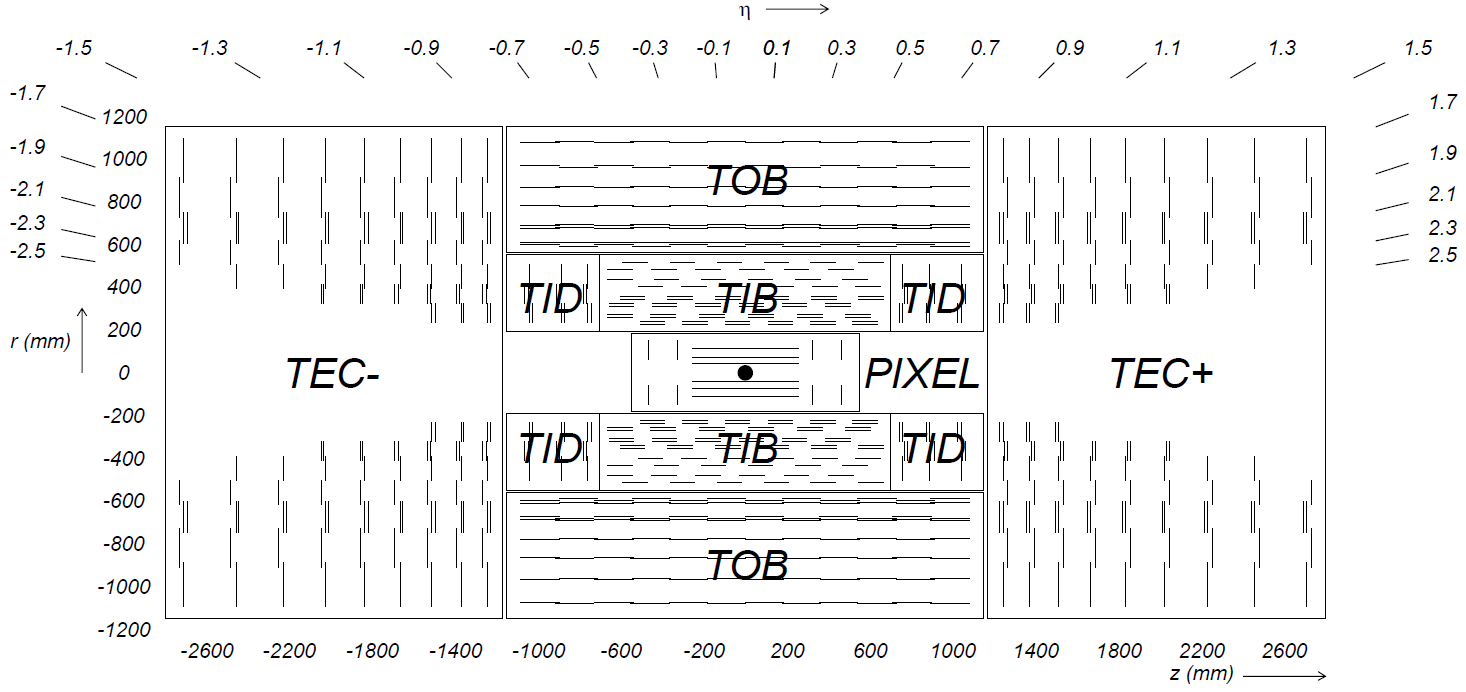
\includegraphics[width=0.1\textwidth]{Images/cmsTracker_TrackerLayout}
\caption{Material budget in units of radiation length as a function of pseudorapidity $\eta$ for the different sub-detectors (left panel) and broken down into the functional contributions (right panel).}
\label{Material_Budget}
\end{figure}
\begin{comment}
% PLOT DELLE PERFORMANCE DEL TRACKER PRESE DAL TDR DEL 2008 --> VANNO MESSE??? VANNO AGGIORNATE???
The tracker has a fundamental role in measuring kinematic variables of the particles: in \figurename~\ref{Tracker_performance_2} is shown the expected resolution of transverse momentum, transverse impact parameter and longitudinal impact parameter, as a function of pseudorapidity for single muons of transerve momentum of 1, 10 and 100 $GeV$. 
\begin{figure}[htbp]
\centering
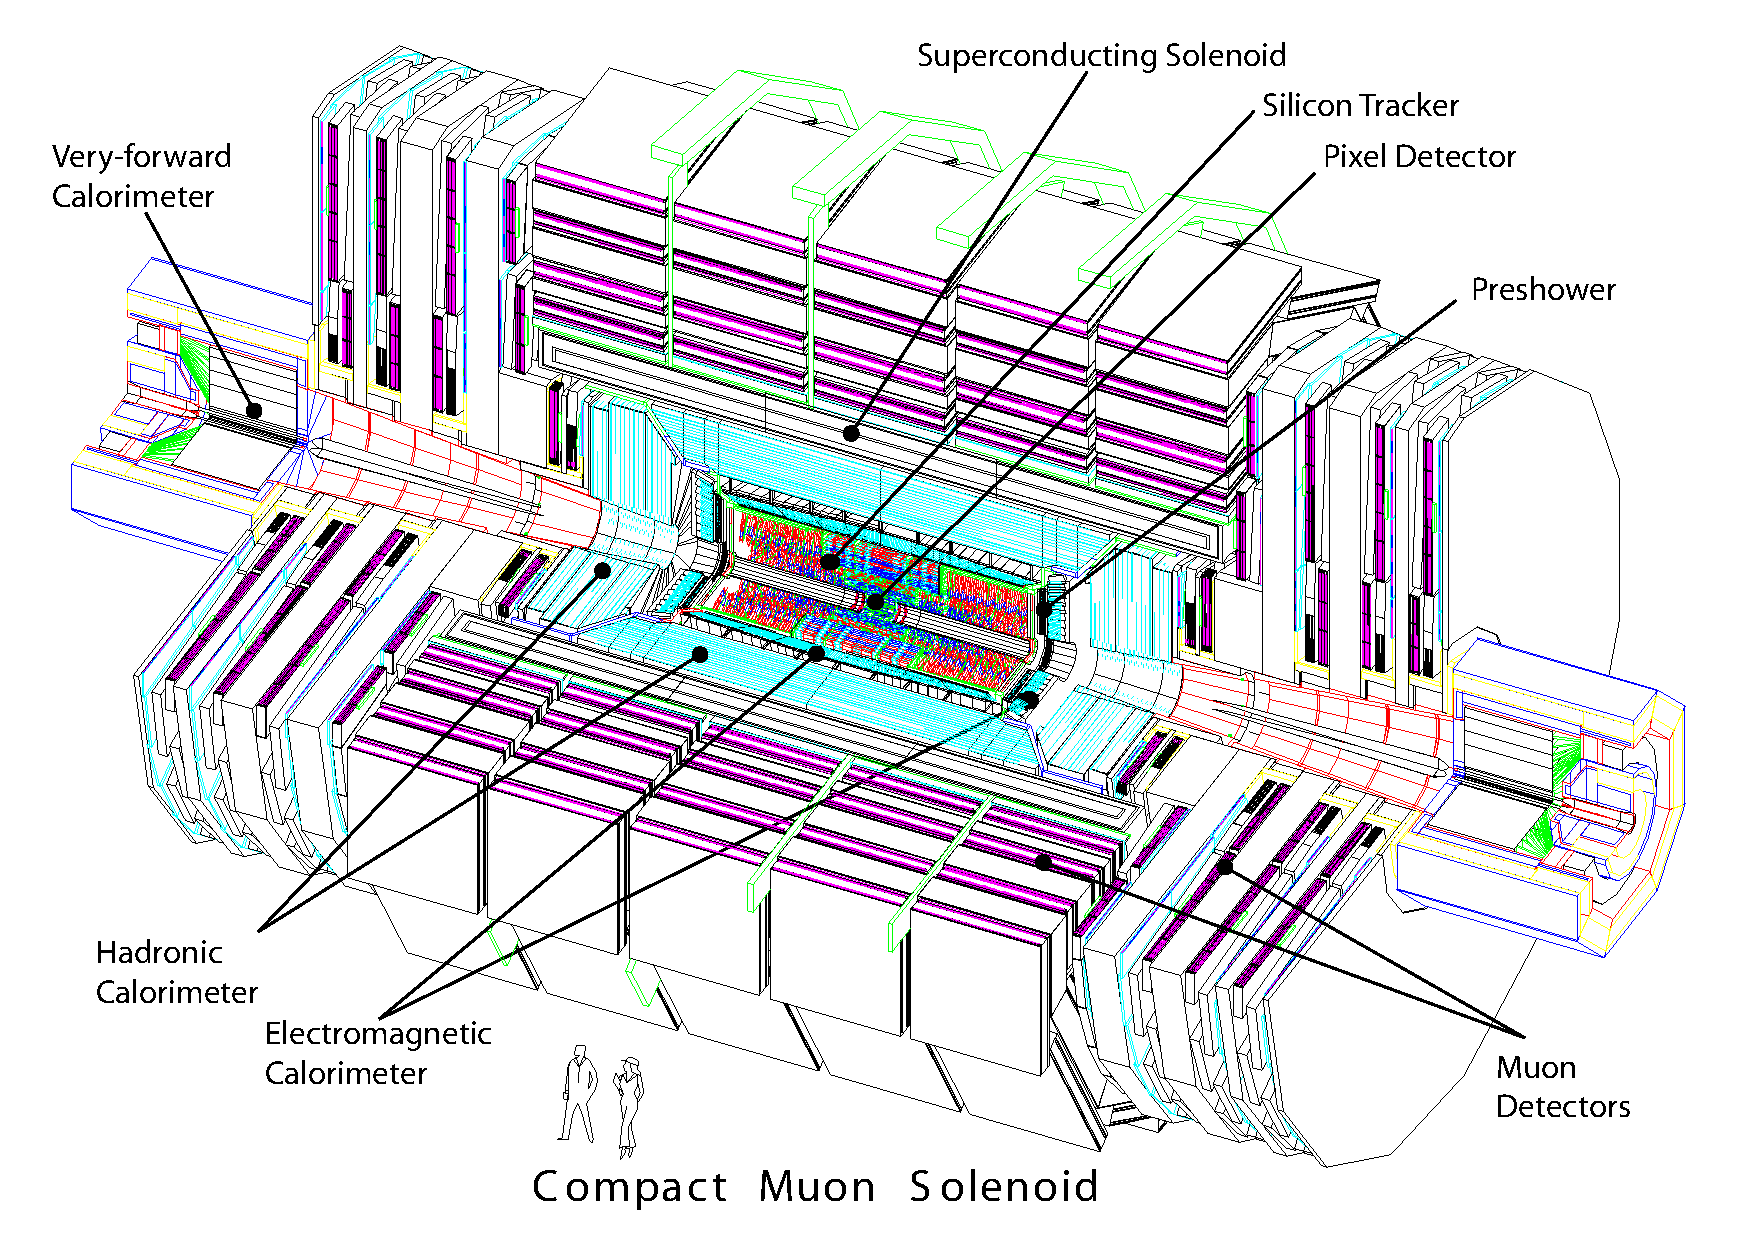
\includegraphics[width=0.1\textwidth]{Images/CMS_Layout.pdf}
\caption{Resolution for single muons with transverse momentum of 1, 10 and 100 GeV for several track parameters: transverse momentum (left panel), transverse impact parameter (middle panel), and longitudinal impact parameter (right panel).}
\label{Tracker_performance}
\end{figure}
For high momentum tracks (100 GeV) the transverse momentum resolution is around 1 - 2\% up to $|\eta| \approx 1.6$, beyond which it degrades due to the reduced lever arm. At a transverse momentum of 100 GeV multiple scattering in the tracker material accounts for 20 to 30\% of the transverse momentum resolution while at lower momentum it is dominated by multiple scattering. The transverse impact parameter resolution reaches 10 $\mu$m for high $p_{T}$ tracks, dominated by the resolution of the first pixel hit, while at lower momentum it is degraded by multiple scattering (similarly for the longitudinal impact parameter). \figurename~\ref{Tracker_performance}  shows the expected track reconstruction efficiency of the CMS tracker for single muons as a function of pseudorapidity: the efficiency is about 99\% over most of the acceptance and it decreases slightly at $|\eta| \approx 0$ due to gaps between the ladders of the pixel detector at z $\approx$ 0. At high $\eta$ the efficiency drop is mainly due to the reduced coverage by the pixel forward disks. \\ 
\begin{figure}[htbp]
\centering
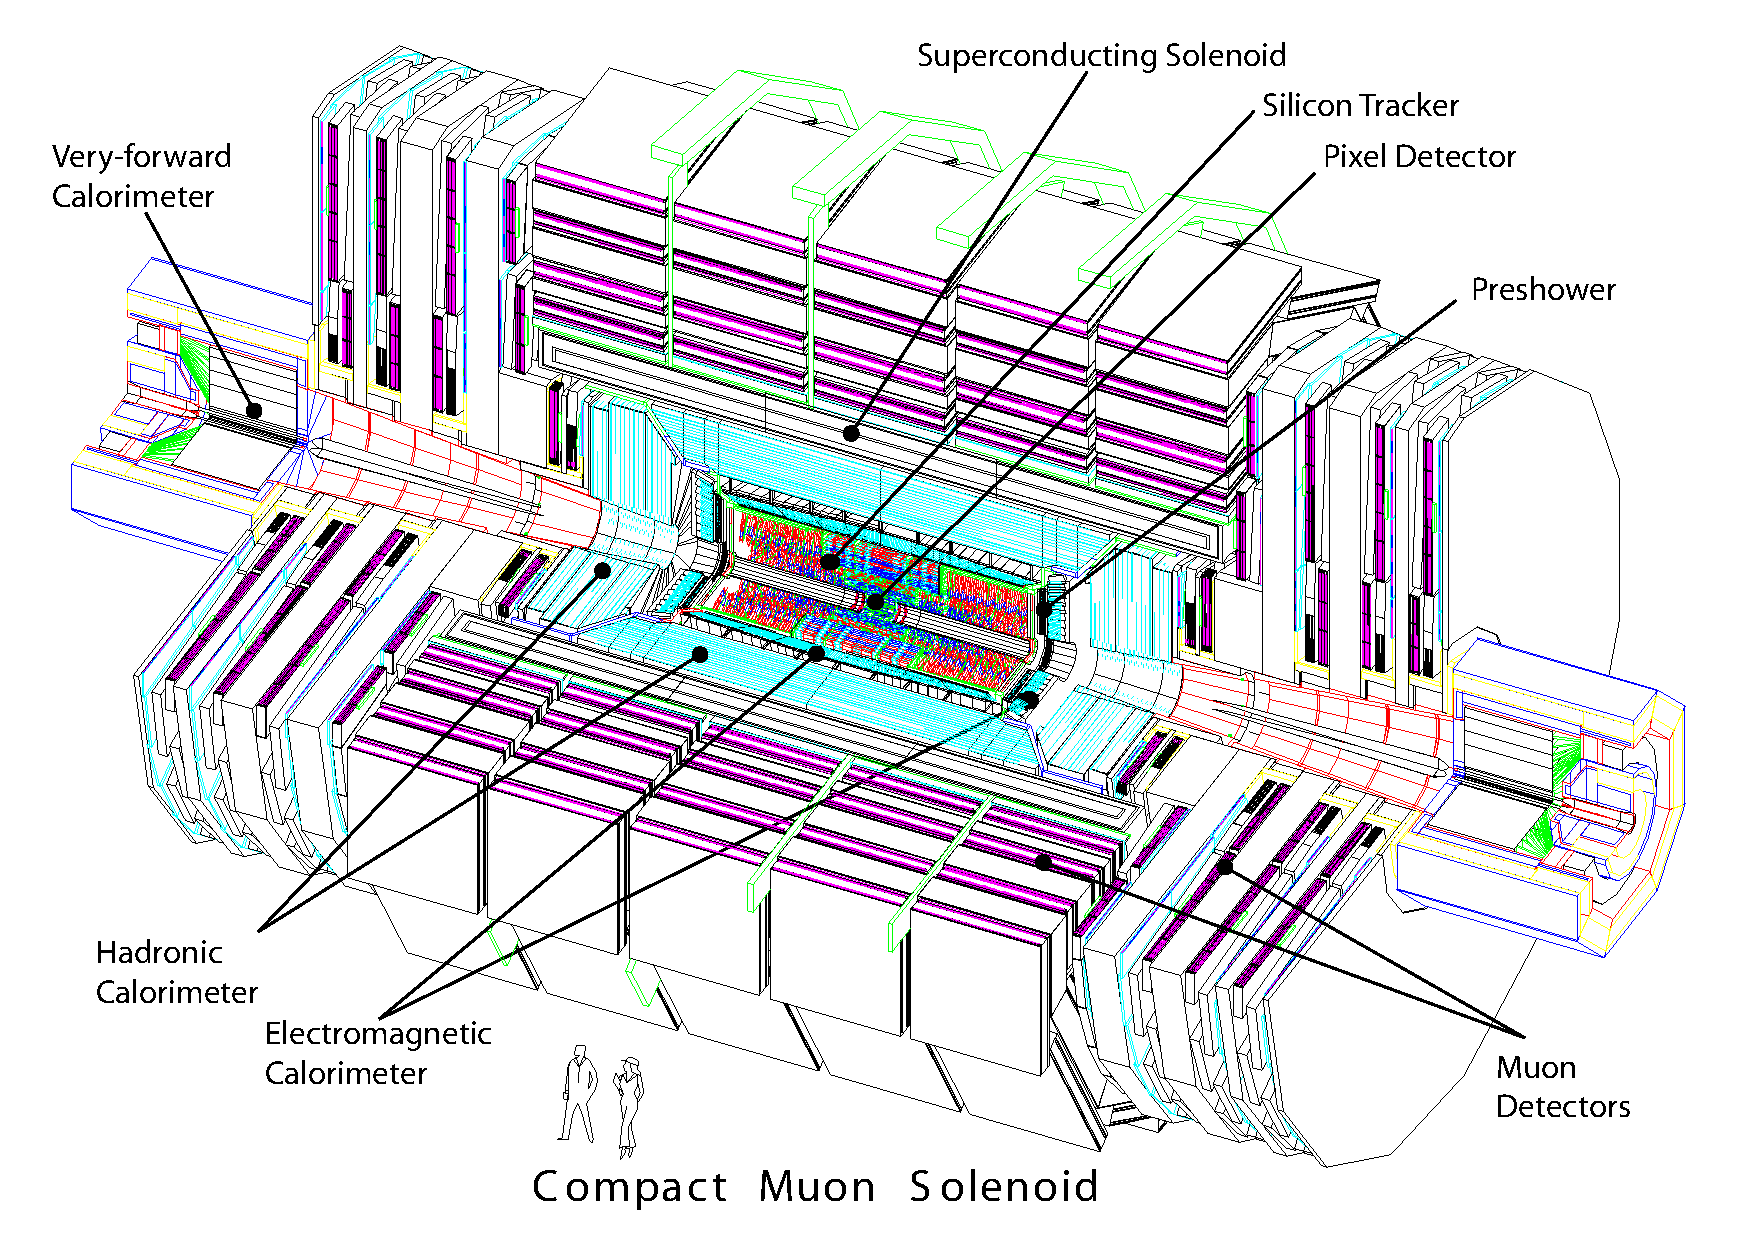
\includegraphics[width=0.1\textwidth]{Images/CMS_Layout.pdf}
\caption{Global track reconstruction efficiency for muons of several transverse momentum: 1, 10, 100 GeV.}
\label{Tracker_performance_2}
\end{figure}
% PLOT DELLE PERFORMANCE DEL TRACKER PRESE DAL TDR DEL 2008 --> VANNO MESSE??? VANNO AGGIORNATE???
\end{comment}

\subsubsection{The pixel detector}
The pixel system is the part of the tracking system that is closest to the interaction region and covers a pseudorapidity range $-2.5 < \eta  < 2.5$, matching the acceptance of the central tracker. \figurename~\ref{Pixel_structure} shows the geometric pixel strcture. It contributes precise tracking points in $r - \phi$ and z and therefore is responsible for a small impact parameter resolution that is important for good secondary vertex reconstruction. With a pixel cell size of $100 \times 150\ \mu m^{2}$ emphasis has been put on achieving similar track resolution in both $r-\phi$ and z directions: 10 $\mu m$ in $r - \phi$ direction and 20 $\mu m$ along z. The pixel detector is essential for the reconstruction of secondary vertices from b and tau decays, and forming seed tracks for the outer track reconstruction and high level triggering. It consists of three barrel layers (BPix) with two endcap disks (FPix). The 53-cm-long BPix layers will be located at mean radii of 4.4, 7.3 and 10.2 cm. The FPix disks, extending from $\approx$ 6 to 15 cm in radius, will be placed on each side at z=$\pm$34.5 and z=$\pm$46.5 cm. BPix (FPix) contain 48 million (18 million) pixels covering a total area of 0.78 (0.28) $m^{2}$. The arrangement of the 3 barrel layers and the forward pixel disks on each side gives 3 tracking points over almost the full $\eta$ range. In the high $\eta$ region the 2 disk points are combined with the lowest possible radius point from the 4.4 cm barrel layer.
\begin{figure}[htbp]
\centering
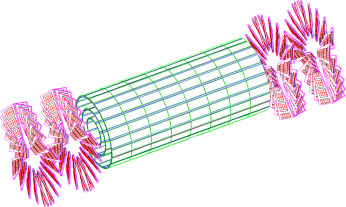
\includegraphics[width=0.5\textwidth]{Images/Pixel_structure}
\caption{Geometrical layout of the pixel detector.}
\label{Pixel_structure}
\end{figure}

\subsubsection{Pixel Upgrade}
Due to the radiation damage and significant data losses due to high occupancy in the readout chip of the pixel detector, the pixel system has been replaced by a new one in the end-of-year shutdown during winter 2016/2017 in order to maintain the excellent tracking and other physics performances \cite{New_Pixel_Detector}. The main new features of the upgraded pixel detector are a ultra-light mechanical design with four barrel layers and three end-cap disks, digital readout chip with higher rate capability and a new cooling system.
\begin{figure}[htbp]
\centering
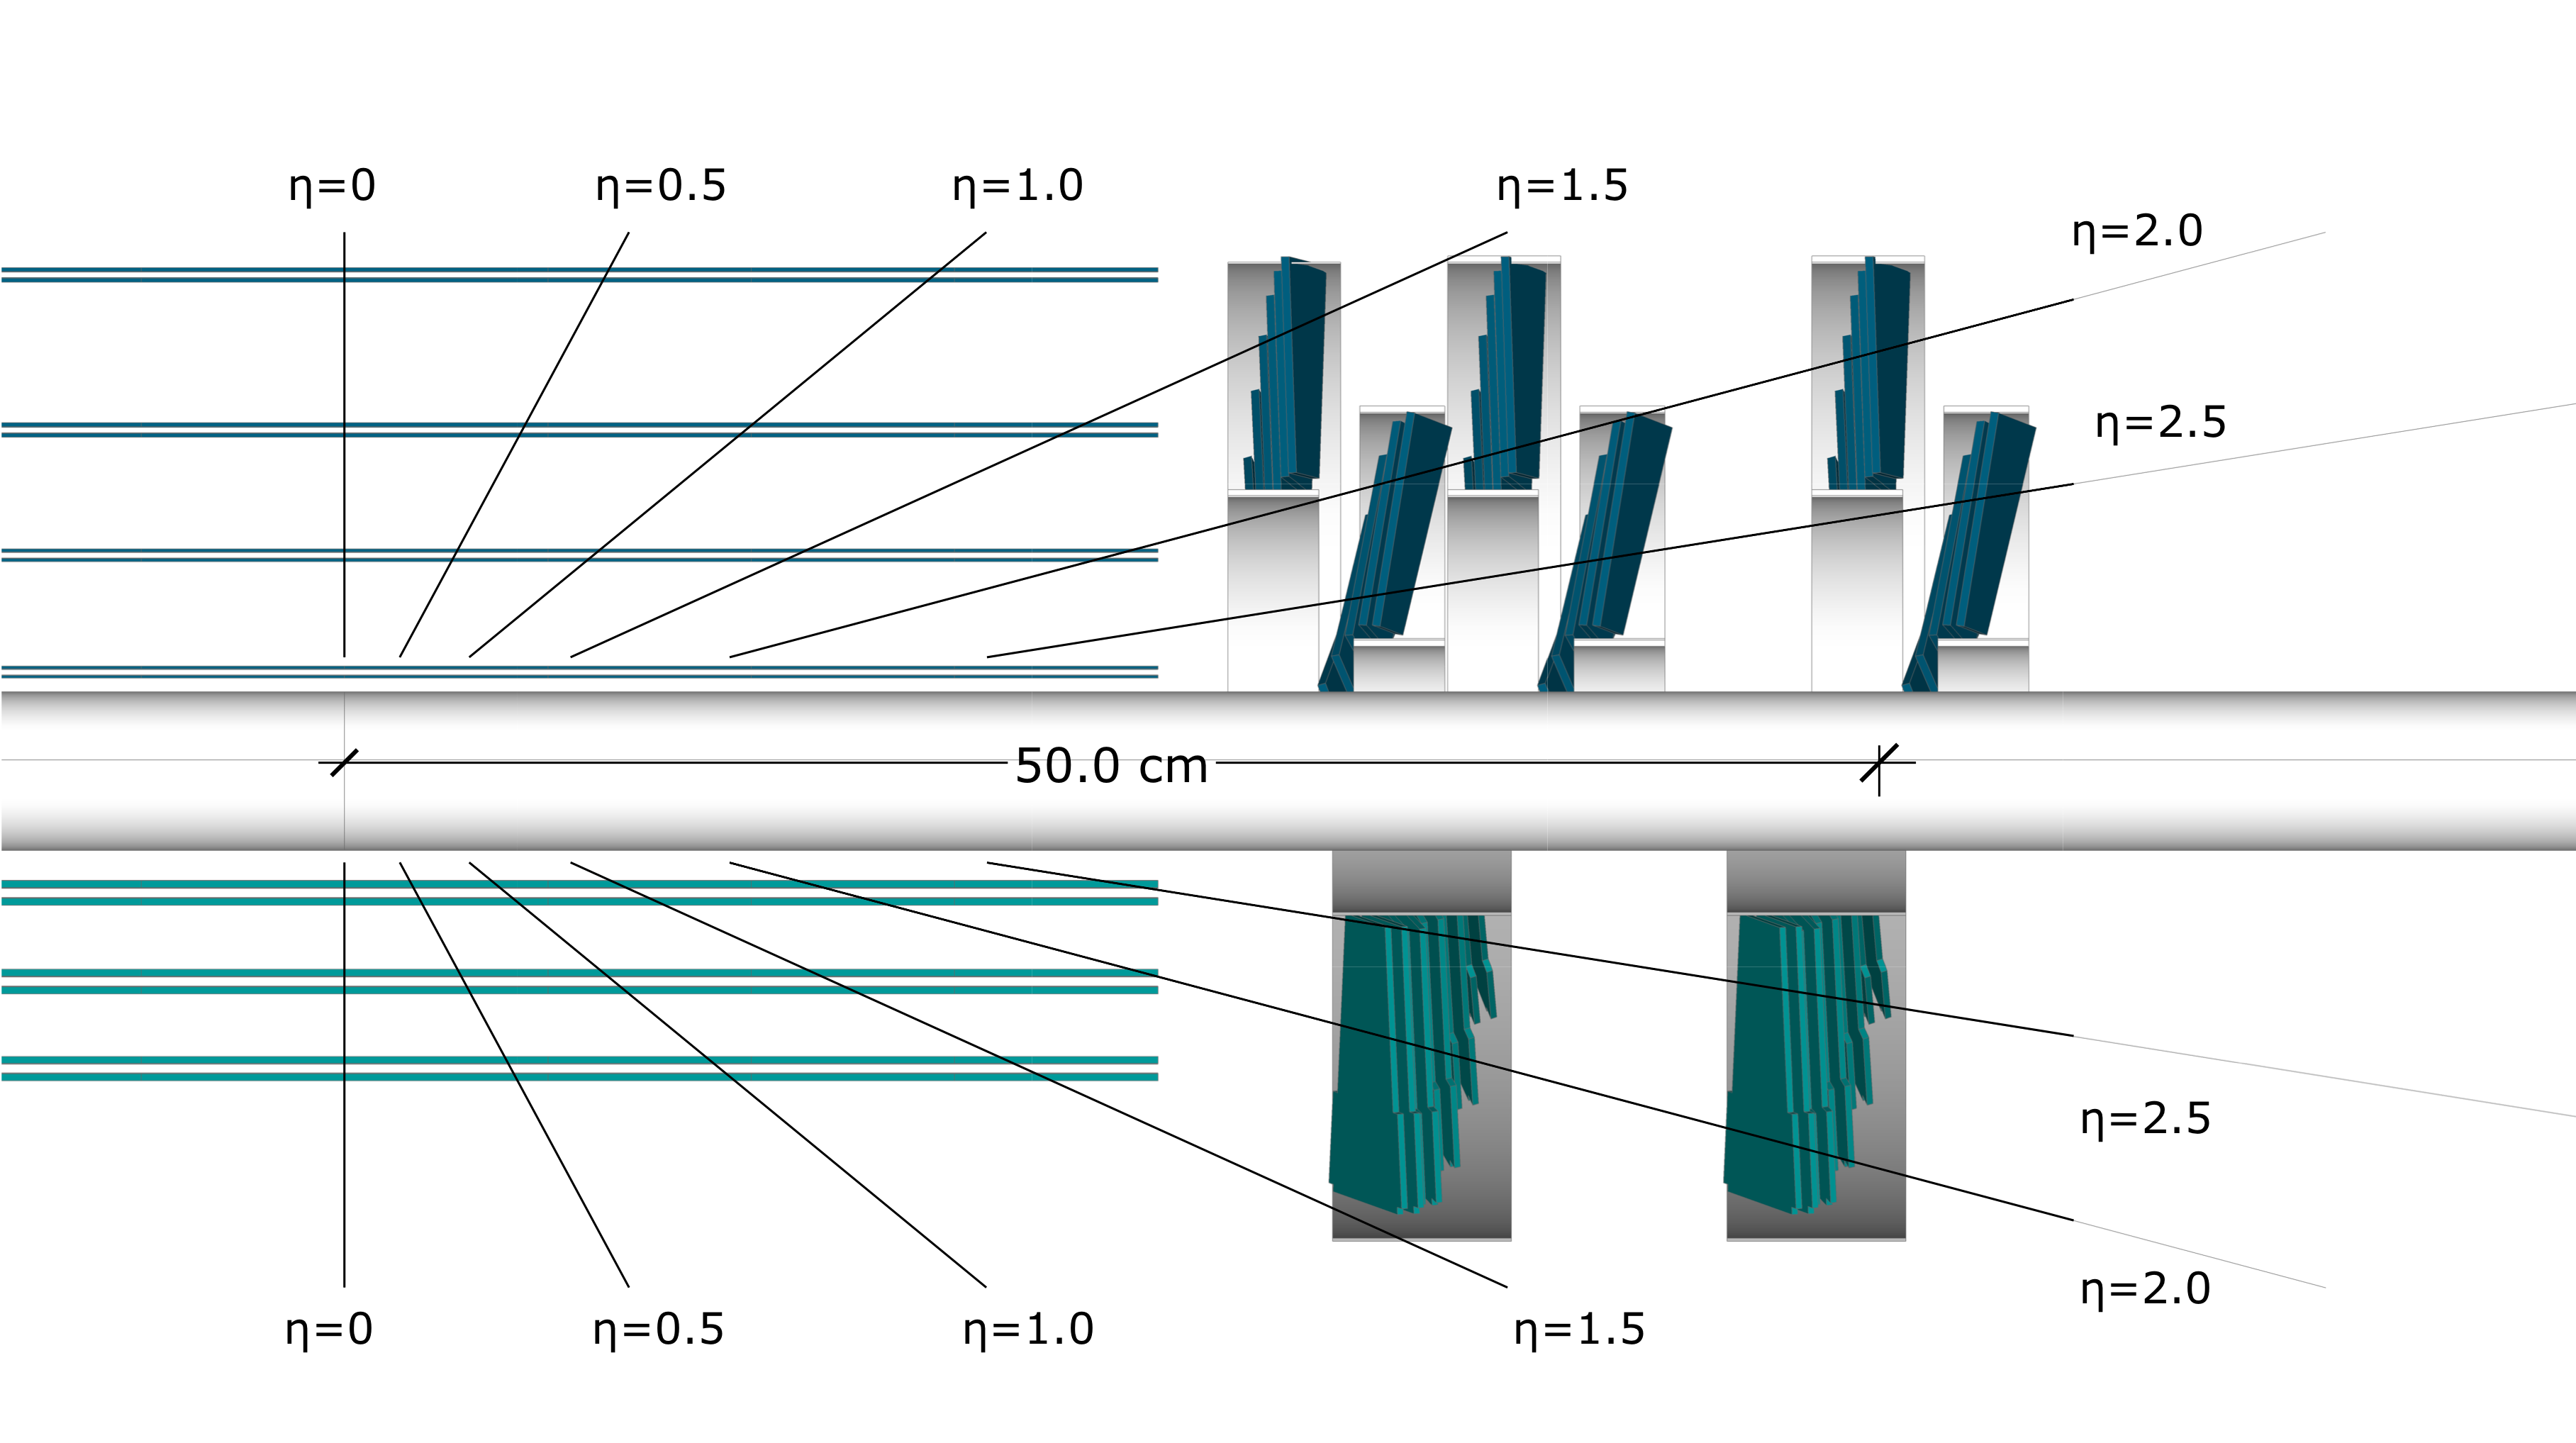
\includegraphics[width=0.65\textwidth]{Images/New_Pixel}
\caption{Comparison of the geometrical layouts of the old (bottom) and upgraded (top) CMS pixel detectors.}
\label{New_Pixel}
\end{figure}
The geometrical layout of the upgrade system, shown in \figurename~\ref{New_Pixel},  consists of four cylindrical barrel layers placed at radii of 29, 68, 109, 160 mm and three disks in each of the forward regions placed at a distance from the nominal interaction point of 291, 396 and 516 mm. This layout is optimized in order to offer full 4-hit tracking coverage up to pseudorapidities of 2.5, with an increased redundancy compared to the present system.

\subsubsection{The silicon strip detector}
The silicon strip detector is composed of three different subsystem. The Tracker Inner Barrel and Disks (TIB/TID  see \figurename~\ref{tracking_system}) are composed of 4 barrel layers, supplemented by 3 disks at each end. TIB/TID delivers up to 4 $r-\phi$ measurements on a trajectory using 320 $\mu m$ thick silicon microstrip sensors with their strips parallel to the beam axis in the barrel and radial on the disks. The strip pitch is 80$\mu m$ on layers 1 and 2 and 120 $\mu m$ on layers 3 and 4 in the TIB, leading to a single point resolution of 23 $\mu m$ and 35 $\mu m$, respectively. In the TID the mean pitch varies between 100$\mu m$ and 141$\mu m$. The TIB/TID is surrounded by the Tracker Outer Barrel (TOB). It has an outer radius of 116 cm and consists of 6 barrel layers of 500$\mu m$ thick microstrip sensors with strip pitches of 183$\mu m$ on the first 4 layers and 122$\mu m$ on layers 5 and 6. It provides another 6 $r-\phi$ measurements with single point resolution of 53$\mu m$ and 35$\mu m$, respectively. The TOB extends in z between $\pm$118cm. Beyond this z range the Tracker EndCaps ($\pm$TEC, where the sign indicates the location along the z axis) cover the region 124 cm $< |z| <$ 282 cm and 22.5 cm $< |r| < $113.5 cm. Each TEC is composed of 9 disks, carrying up to 7 rings of silicon microstrip detectors (320$\mu m$ thick on the inner 4 rings, 500$\mu m$ thick on rings 5-7) with radial strips of 97$\mu m$ to 184$\mu m$ average pitch. Thus, they provide up to 9 $\phi$ measurements per trajectory. In addition, the modules in the first two layers and rings, respectively, of TIB, TID, and TOB as well as rings 1, 2, and 5 of the TECs carry a second microstrip detector module which is mounted back-to-back with a stereo angle of 100 mrad in order to provide a measurement of the second coordinate (z in the barrel and r on the disks). The achieved single point resolution of this measurement is 230$\mu m$ and 530$\mu m$ in TIB and TOB, respectively, and varies with pitch in TID and TEC. \\
The sensor elements in the strip tracker are single sided p-on-n type silicon micro-strip sensors shown in \figurename~\ref{Silicon_structure}: in TIB/TID and on the inner 4 rings of the TECs, thin sensors of (320 $\pm$ 20) $\mu m$ wafer thickness are used, with substrate resistivity of $ro$ = 1.55 - 3.25 k$\Omega$cm; TOB and the outer 3 rings of the TECs are equipped with thicker sensors of (500 $\pm$ 20) $\mu m$ thickness, with substrate resistivity of $ro$ = 4 - 8 k$\Omega$cm. 
\begin{figure}[htbp]
\centering
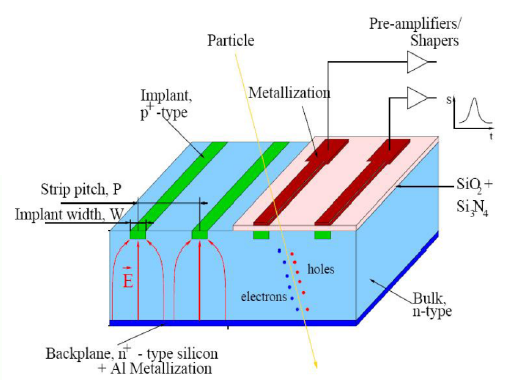
\includegraphics[width=0.35\textwidth]{Images/Silicon_structure}
\caption{Single sided p-on-n type silicon micro-strip sensor.}
\label{Silicon_structure}
\end{figure}

LASER ALIGNMENT SYSTEM

\subsection{Electromagnetic calorimeter}
The electromagnetic calorimeter plays an essential role in the study of the physics of electroweak symmetry breaking, and  in the exploration of  beyond the Standard Model scenarios.  ECAL is a homogeneous calorimeter of almost 76000 Lead Tungstate $PbWO_4$ scintillating crystals divided into a barrel and two endcaps.
A $3$D view of the barrel and endcap electromagnetic calorimeter is shown in \figurename~\ref{ECAL_3D}.
\begin{figure}[h!]
 \centering
 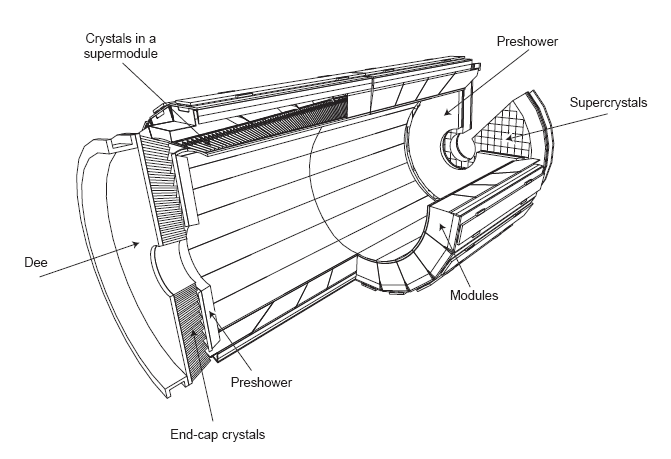
\includegraphics[width=0.75\textwidth]{Images/ECAL_3D}
 \caption{A $3$D view of the electromagnetic calorimeter.}
\label{ECAL_3D}
\end{figure}


\subsubsection{The Barrel Calorimeter}
The barrel part of the ECAL covers the pseudorapidity range $|\eta| < 1.479$ 
%(see Figure~\ref{fig:ecalSection}). 
The front face of the crystals is at a radius of $1.29 \,$m and each crystal has a square cross-section of $ 22 \times 22 \,$mm$^2$ and a length of $230 \,$mm corresponding to $25.8 \,$X$_0$. The truncated pyramid-shaped crystals are mounted in a geometry which is off-pointing with respect to the mean position of the primary interaction vertex, with a $3^{\circ}$ tilt in both $\phi$ and in $\eta$. The crystal cross-section corresponds to $\Delta \eta \times \Delta \phi = 0.0175 \times 0.0175$ ($1^{\circ}$). 
\begin{comment}
\begin{figure}[h!]
 \centering
 \includegraphics[width=0.80\textwidth]{cms/img/ecalTDR/longitudinal-view-16.pdf}
 \caption[ECAL longitudinal section]{Longitudinal section of the electromagnetic calorimeter (one quadrant)}
\label{fig:ecalSection}
\end{figure}
\end{comment}
The barrel granularity is $360$-fold in $\phi$ and ($2 \times 85$)-fold in $\eta$, resulting in a total number of $61\,200$ crystals. The crystal volume in the barrel amounts to $8.14 \,$m$^3$ ($67.4 \,$t). Crystals for each half-barrel are grouped in $18$ supermodules each subtending $20^{\circ}$ in $\phi$. Each supermodule comprises four modules with $500$ crystals in the first module and $400$ crystals in each of the remaining three modules. For simplicity of construction and assembly, crystals have been grouped in arrays of $2 \times 5$ crystals which are contained in a very thin wall ($200 \,\mathrm{\mu m}$) alveolar structure and form a submodule.  Thermal regulation is carried out by two active systems: 1) a specially regulated cooling circuit which keeps the operating temperature (ambient temperature) of the crystal array and of the APDs within a tight temperature spread of $\pm0.05 \, ^{\circ}$C, ensuring adequate thermal stability; 2) the power cooling circuit evacuates the heat generated by all power sources in the supermodule (each supermodule is designed as a separate thermal entity).

\begin{comment}
\subsection{The Endcap Calorimeter}

The endcap part of the crystal calorimeter covers a pseudorapidity
range from $1.48$ to $3.0$. The design of the endcaps provides precision
energy measurement up to $|\eta| = 2.5$. Crystals are however installed
up to $|\eta| = 3$ in order to augment the energy-flow measurement in
the forward direction.  The mechanical design of the endcap calorimeter
is based on an off-pointing pseudo-projective geometry using tapered
crystals of the same shape and dimensions ($24.7 \times 24.7 \times 220 \,$mm$^3$)
grouped together into units of $36$, referred to as supercrystals. A
total of $268$ identical supercrystals is used to cover each
endcap with a further $64$ sectioned supercrystals used to complete
the inner and outer perimeter. Each endcap contains 7324 crystals,
corresponding to a volume of $1.52 \,$m$^3$ ($12.6 \,$t). Both endcaps are
identical. Each endcap detector is constructed using Dee-shaped
sections as seen in Figure~\ref{fig:EE}. 
\begin{figure}[h!]
 \centering
 \includegraphics[width=0.50\textwidth]{cms/img/ecalTDR/endcap-18.pdf}
 \caption{A single endcap with Dees apart.}
\label{fig:EE}
\end{figure}

Figure~\ref{fig:materialBudget} shows the total thickness (in radiation
lengths) of the ECAL as a function of pseudorapidity. The
endcap part also includes the preshower detector.  
\begin{figure}[h!]
 \centering
 \includegraphics[width=0.50\textwidth]{cms/img/ecalTDR/material-budget-17.pdf}
 \caption[ECAL thickness in X$_0$]{Total thickness in X$_0$ of the ECAL as a function of pseudorapidity, averaged over $\phi$.}
\label{fig:materialBudget}
\end{figure}
Because of the
high radiation levels in the endcaps all materials
used in this region must tolerate very large doses and neutron fluences.  



\subsection{The Preshower Detector} 

The endcap preshower covers a pseudorapidity range
from $|\eta| = 1.65$ to $2.61$. 
Its main function is to provide $\pi^{0}$-$\gamma$ separation. 
The preshower detector, placed
in front of the crystals, contains two lead converters of a total
thickness of $2 \,$X$_0$ and $1 \,$X$_0$ respectively, followed by detector
planes of silicon strips with a pitch of $< 2 \,$mm. The impact position
of the electromagnetic shower is determined by the center-of-gravity
of the deposited energy. The accuracy is typically $300 \,\mathrm{\mu m}$ at 
$50 \,$ GeV. In order to correct for the energy deposited in the lead
converter, the energy measured in the silicon is used to apply
corrections to the energy measurement in the crystal. The fraction
of energy deposited in the preshower (typically $5\%$ at $20 \,$ GeV)
decreases with increasing incident energy.
Figure~\ref{fig:ES} shows the
layout of the preshower.
\begin{figure}[h!]
 \centering
 \includegraphics[width=0.80\textwidth]{cms/img/ecalTDR/es-19.pdf}
 \caption{Schematic section through the endcap preshower.}
\label{fig:ES}
\end{figure}

To maintain its performance during the lifetime of the experiment,
the endcap silicon detector has to be operated at $-5 \, ^{\circ}$C. Heating
films and insulating foam glued on the moderators guarantee that
the external surfaces are kept at the ambient temperature of the
neighboring detectors.


\subsection{Lead Tungstate Crystals}
The characteristics 
of the Lead Tungstate crystals (PbWO$_4$) make them an appropriate choice for operation at LHC~\cite{Beringer:1900zz}. The high density ($8.3 \,$g/cm$^3$), short radiation length ($0.89 \,$cm) and small
Moli\`ere radius ($2.2 \,$cm) results in a fine granularity and a compact
calorimeter. The scintillation decay time is of the same order of
magnitude as the LHC bunch crossing time: about $80\%$ of the light
is emitted in $25 \,$ns. The light output is relatively low: about $4.5$
photoelectrons per MeV are collected in both the avalanche photodiodes
(APDs) and the vacuum phototriodes (VPTs), where the higher APD
quantum efficiency is balanced by their smaller surface coverage
on the back face of the crystal. The crystals emit blue-green
scintillation light with a broad maximum at $420\,$nm~\cite{Annenkov:200230}. 


\subsection{Amplitude reconstruction}\label{sec:amplitude}
The raw data for a single channel consists of a series of consecutive digitization 
of the signal making up a time frame\cite{1748-0221-5-03-T03011}. The number of samples is adjustable (2+4n) with a default of 10. 
The digitizations are made at the bunch crossing frequency of 40 MHz, i.e. one sample each 25 ns.
 In addition, the timing of the signal is adjusted in LHC running so that the signal pulse maximum corresponds to one of the samplings. 
 Figure \ref{fig:ampl} shows an example of the time sampling for a signal pulse as a function of the time difference $(T-T_{max})$, 
 where $T$ and $T_{max}$ indicate the time of the generic ADC sample and the time corresponding to the maximum of the pulse shape respectively.
 \begin{figure}[h!]
 \centering
 \includegraphics[width=0.75\textwidth]{cms/img/ampl.png}
 \caption{Pulse shape measured in the ECAL as a function of $(T-T_{max})$.}
\label{fig:ampl}
\end{figure}
The simplest method of reconstructing the amplitude of the channel is to take the sampling on the maximum as
 the measurement of the signal. However, a larger number of samples is preferred since it allows more sophisticated digital 
 processing of the signal to reduce noise contribution. The other reason is to enable the identification of pile-up events from other bunch crossing.
The signal amplitude is computed as a linear combination of discrete time samples:
\begin{equation}
 A= \sum_{i=0}^N S_i \times w_i
 \end{equation}
where $w_i$ are the weights, $S_i$ the time sample values in ADC counts and $N$
  is the number of samples used in the filtering. The weights are determined to minimize the noise contribution.
Amplitude and time measurement are strongly correlated. After a signal has been amplified and shaped by the
   front-end electronics, the channel timing reconstruction consists in a precise measurement of the time the 
   pulse reaches its maximum values $A_{max}$. Looking at Figure \ref{fig:ampl}, the reconstructed time of a 
   channel corresponds to the value of $T_{max}$. 


\subsection{Energy Resolution}
For the energy range of
about $25$ GeV  to $500$ GeV, the ECAL energy resolution has been parameterized 
as: 
\begin{equation}
 \frac{\sigma(E)}{E} =  \frac{a}{\sqrt{E}} \oplus \frac{\sigma_n}{E} \oplus c \quad \text{(E in GeV)}
\end{equation}
 where $a$ is the
stochastic term, $\sigma_n$ the noise, and $c$ the constant term. 
Figure~\ref{fig:resolution-ecal} summarizes the different
contributions expected for the energy resolution. Terms representing
the degradation of the energy resolution at extremely high energies
have not been included. The stochastic
term includes fluctuations in the shower containment as well as a
contribution from photostatistics.  The noise term contains the contributions
from electronic noise and pile-up energy; the former is quite important
at low energy, the latter is negligible at low luminosity. The curve
labeled \textit{intrinsic} includes the shower containment and a constant
term of $0.55\%$. The constant term must be kept down to this level
in order to profit from the excellent stochastic term of PbWO$_4$ in
the energy range relevant for the search for new physics. To achieve this
goal, in situ calibration/monitoring using isolated high $p_T$ electrons
is performed.  
\begin{figure}[h!]
 \centering
 \includegraphics[width=0.85\textwidth]{cms/img/ecalTDR/resolution-13.pdf}
 \caption[Resolution of the PbWO$_4$ calorimeter]{Different contributions to the energy resolution of the PbWO$_4$ calorimeter.}
\label{fig:resolution-ecal}
\end{figure}

\subsection{ECAL Time measurement and resolution}
The algorithm used to extract $T_{max}$ relies on an alternative representation of the pulse shape, 
provided by a a variable defined as the ratio between the amplitudes of two consecutive samples\cite{1748-0221-5-03-T03011}:
\begin{equation}
R(T)=\frac{A(T)}{A(T+25ns)}
\end{equation}
where $A(T)$ represents the pulse amplitude at time $T$ . Figure \ref{fig:ration} illustrates the parametrization of time difference $(T-T_{max})$ as a function of $R(T)$.
 In view of the universal character of the pulse shape, this representation is independent on the maximum amplitude $A_{max}$
  and can be described well with a simple polynomial parametrization.
  \begin{figure}[h!]
 \centering
 \includegraphics[width=0.65\textwidth]{cms/img/ration.png}
 \caption{Time difference $(T-T_{max})$ as a function of the ratio of the amplitudes $R (T )$. }
\label{fig:ration}
\end{figure}

Each pair of consecutive samples gives a measurement of the ratio: 
 \begin{equation}
R_i=\frac{A(T+[i]\cdot 25ns)}{A(T+[i+1]\cdot25ns)}
\end{equation}
An estimate $T_{max,i}$ of the maximum time can be obtained from each $R_i$ ratio as $T_{max,i} = T_i-T (R_i)$. 
A more precise determination of the maximum time and its uncertainty is then obtained from the weighted average of the estimated $T_{max,i}$:
\begin{equation}
T_{max}=\frac{\sum_i \frac{T_{max,i}}{\sigma^2_i}}{\sum_i \frac{1}{\sigma^2_i}}
\end{equation}

\begin{equation}
\frac{1}{\sigma^2_T}=\sum_i \frac{1}{\sigma^2_i}
\end{equation}
The typical number of available ratios $R_i$ is five or six.

To determine the intrinsic time resolution of the ECAL, electrons from a test
beam with energy between 15 and 300 GeV are used.
 The time resolution is extracted from the distribution of the time difference
  between adjacent crystals that share the same electromagnetic shower and measure similar energies.
   The distribution of the time difference is well described by a Gaussian function, whose width can be parametrized as \cite{1748-0221-5-03-T03011}:
 \begin{equation}
\sigma^2(t_1-t_2) = \left ( \frac{N\sigma_n}{A_{eff}} \right)^2+C^2
\end{equation}  
where $A_{eff} = E_1E_2/\sqrt{E_{1}^2 + E_2^2}$, with $t_{1,2}$ and $E_{1,2}$
 corresponding to the times and energies measured in the two crystals, $\sigma_n$ is a parameter related to the noise level, 
 $N$ and $C$ represent the noise and constant term coefficients of time resolution. 
 The extracted width is presented in Figure \ref{fig:timereso} as a function of the variable $A_{eff}/\sigma_n$. 
 The energy scales for barrel and endcap are superimposed in the plot.
 \begin{figure}[h!]
 \centering
 \includegraphics[width=0.65\textwidth]{cms/img/timereso.png}
 \caption{ Gaussian width of the time difference between two neighboring crystals as a function of the variable $A_{eff}/\sigma_n$,
  for test beam electrons between 15 and 300 GeV. The equivalent single-crystal energy scales for barrel and endcaps are overlaid on the plot.}
\label{fig:timereso}
\end{figure}

Precise ECAL time determination results to be crucial in many respects.
The better the precision of time measurement and synchronization, 
the larger the rejection of backgrounds with a broad time distribution.
 Such backgrounds are cosmic rays, beam halo muons, electronic noise, and out-of- time proton-proton interactions.
  Precise time measurement also makes it possible to identify particles predicted by different models beyond the Standard Model. 
  Slow heavy charged R-hadrons \cite{Chatrchyan:2013oca}, which travel through the calorimeter and interact before decaying, 
  and photons from the decay of long-lived new particles that reach the calorimeter out-of-time with respect
   to particles travelling at the speed of light from the interaction point. To achieve these goals the time measurement performance both at low energy (1 GeV or less) and high energy (several tens of GeV) for showering photons have been studied also with collision data in order to reproduce the results obtained at the test beam.
    Indeed during collisions several effects can worsen significantly the design resolution, as for example, run by run variations, inter-calibration, effects vs energy, radiation, the presence of the  magnet field and of the tracker material in front of the ECAL. The time resolution estimated with 8 TeV data, looking at the time difference of electrons produced in the decay of a Z boson in CMS, is shown in Figure \ref{fig:timerescol}. The noise term results to be consistent with the one obtained at the test beam, while the constant term is about 150 ps. This value although far from the design performance, it is almost ok for every physics application.
An example of the use of the ECAL time measurement in physics analysis is presented in appendix \ref{app:neut}. In this analysis, for the first time, the novel technique of exploiting
 the ECAL time measurement is used to identify off time photons produced in the decays of long-lived neutralinos, with decay lengths comparable to the ECAL radial size.
  
   \begin{figure}[h!]
 \centering
 \includegraphics[width=0.65\textwidth]{cms/img/timerescol.png}
 \caption{ Gaussian width of the time difference between two electrons produced in the decay of a Z boson as a function of the variable $A_{eff}/\sigma_n$.
The equivalent single-crystal energy scales for barrel and endcaps are overlaid on the plot.}
\label{fig:timerescol}
\end{figure}

  
\section{Magnet}
The required performance of the muon system, and hence the bending power, is defined
by the narrow states decaying into muons and by the unambiguous determination of the
sign for muons with a momentum of $ 1\,$ TeV/c. This requires a momentum resolution of $\Delta p / p \sim 10 \%$ at $p = 1$ TeV. 

To achieve this goal, CMS chose a large superconducting solenoid, the parameters of which are given in table~\ref{tab:magnetParameters}. 

\begin{table}[h!]
\centering

 \begin{tabular}{ l  c }
\toprule
Parameter & Value \\
  \midrule
  Field & $3.8\,$T \\
  Inner bore & $5.9 \,$m \\
  Length & $12.9 \,$m \\
  Number of turns & $2168$ \\
  Current & $19.5 \,$kA \\
  Stored energy & $2.7 \,$GJ\\
  \bottomrule
 \end{tabular}
 \caption{Parameters of the CMS superconducting solenoid.}
\label{tab:magnetParameters}
\end{table}



%\begin{figure}[ht]
\begin{figure}[h!]
 \centering
 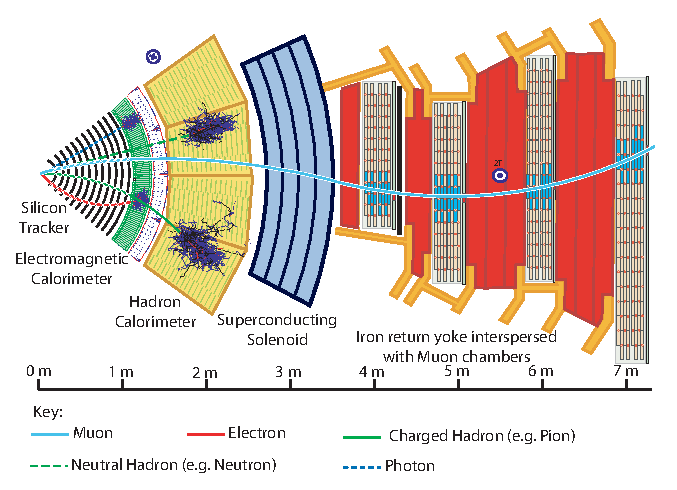
\includegraphics[width=0.85\textwidth]{cms/img/cms_slice.pdf}
 \caption{Schematic view of a transverse slice of the central part of the CMS detector.}
\label{fig:cmsSection}
%\end{figure}
\end{figure}
 



\section{Hadron Calorimeter}
\label{sec:HCAL}

The design of the hadron calorimeter (HCAL) \cite{CMS:1997tfa} is strongly influenced by the choice of the magnet parameters since most of the CMS calorimetry is located inside the magnet coil and surrounds the ECAL system (see figure~\ref{fig:cmsSection}). An important requirement of HCAL is to minimize
the non-Gaussian tails in the energy resolution and to provide good containment and hermeticity. Hence, the HCAL design maximizes material inside the magnet coil in terms of interaction lengths. This is complemented by an additional layer
of scintillators, referred to as the hadron outer (HO) detector, lining the outside of the coil.
Brass has been chosen as absorber material as it has a reasonably short interaction length,
is easy to machine and is non-magnetic. Maximizing the amount of absorber before the magnet requires minimizing the amount of space devoted to the active medium. The tile/fiber technology makes for an ideal choice. It consists of plastic scintillator tiles read
out with embedded wavelength-shifting (WLS) fibers. The WLS fibers are spliced to high-attenuation-length clear fibers are just outside the scintillator carrying the light to the readout system. 
The photodetection
readout is based on multi-channel hybrid photodiodes (HPDs). The absorber structure is assembled by bolting together precisely machined and overlapping brass plates so as to leave space to insert the scintillator plates, which have a thickness of $3.7 \,$mm. The overall assembly
enables the HCAL to be built with essentially no uninstrumented cracks or dead areas in $\phi$.
%The gap between the barrel and the endcap HCAL, through which the services of the ECAL
%and the inner tracker pass, is inclined at $53^{\circ}$ and points away from the center of the detector.


\section{Muon System}
The muon system is the outermost of the CMS subdetectors. Its main goals are the identification of muons, thanks to their high penetrating power, and
a precise measurement of their momentum, with the help of the information
coming from the tracker. The muon system also works as trigger for events
which involve muons and it provides a precise time measurement of the bunch
crossing.
The CMS muon system \cite{muon} relies on three kinds of gaseous detectors:
drift tubes (DT), cathode strip chambers (CSC) and resistive plate chambers
(RPC). The DT and the CSC provide an excellent spatial resolution for the measurement of charged particle momentum; the RPC are
used for trigger issues because of the very good timing. The active parts of
the muon system are hosted into stations which are interleaved by the iron
layers of the return yoke of the magnet. The longitudinal view of a quarter of
the muon system is given in Figure \ref{fig:muon}. The barrel extends up to $|\eta|<1.4$,
the endcaps up to $|\eta|<2.4$. 
\begin{figure}[h!]
 \centering
 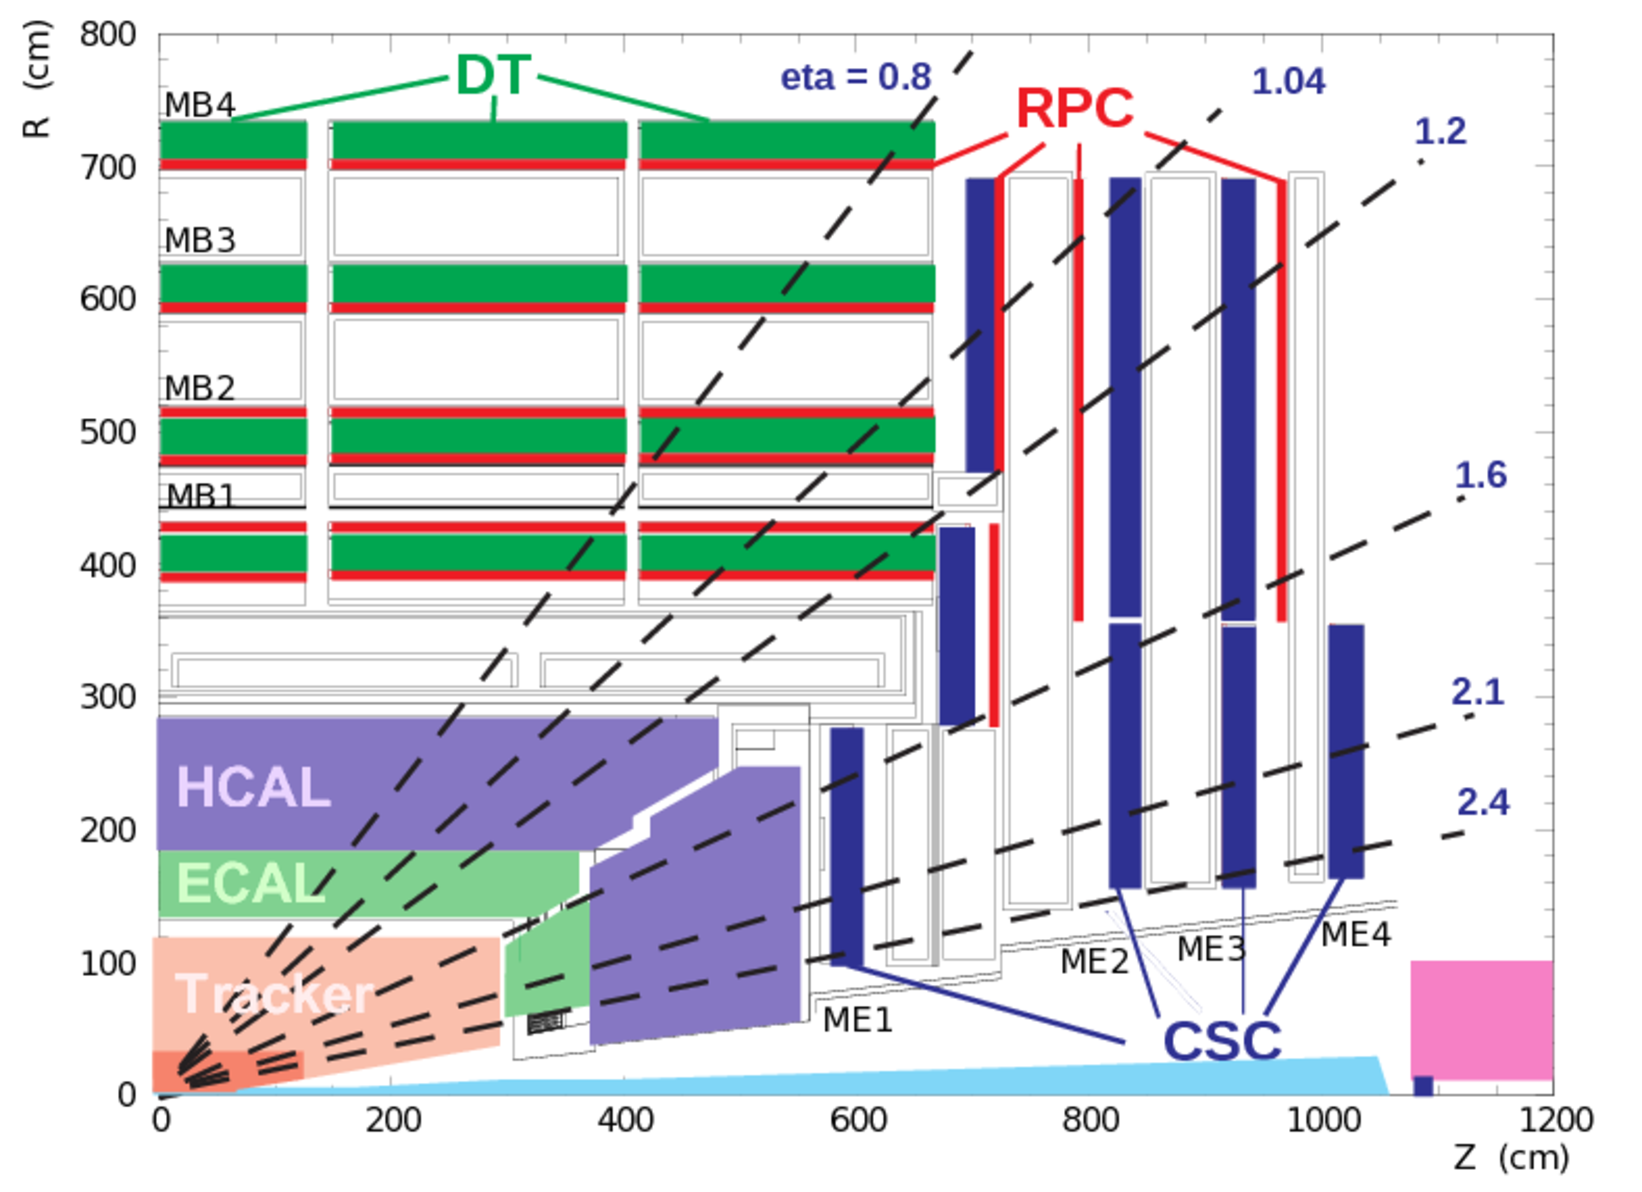
\includegraphics[width=0.85\textwidth]{cms/img/muonsyst.pdf}
 \caption{Longitudinal view of one quarter of the CMS muon system}
\label{fig:muon}
%\end{figure}
\end{figure}
 

\section{Trigger and Data Acquisition}\label{sec:trig}

The trigger system in CMS is the start of the physics event selection process. A
decision to retain an event for further consideration has to be
made every $25 \,$ns. This decision is based on the event's suitability
for inclusion in one of the various datasets to be used for analysis.
The datasets to be taken are determined by CMS physics priorities
as a whole. These datasets include dilepton and multilepton datasets, diphoton datasets,
lepton plus jet datasets for top, Higgs and BSM physics, and inclusive electron datasets for calorimeter calibrations.
In addition, other samples are necessary for measuring efficiencies
in event selection and studying backgrounds. The trigger has to
select these samples in real time along with the main data samples.

For the nominal LHC design luminosity of $10^{34} \,$cm$^{-2}$s$^{-1}$, an average
of $17$ events occurs at the beam crossing frequency of $25$ ns. This
input rate of $10^9$ interactions every second must be reduced by a
factor of at least $10^7$ to $100 \,$Hz, the maximum rate that can be
archived by the on-line computer farm. CMS has chosen to reduce
this rate in two steps. At the first level (L1) all data is stored for
$3.2 \, \mathrm{\mu s}$, after which no more than $100 $\,kHz of the stored events are
forwarded to the High Level Triggers (HLT). The L$1$ system uses only coarsely segmented
data from calorimeter and muon detectors, while holding all the
high-resolution data in pipeline memories in the front-end electronics.
The HLT is provided by a subset of the on-line processor farm which,
in turn, passes a fraction of these events to the remainder of the
on-line farm for more complete processing.





\subsection{Level $1$ Trigger}

The design of the CMS Trigger and Data Acquisition system is illustrated in figure~\ref{fig:trigger}.
\begin{figure}[h!]
\centering
 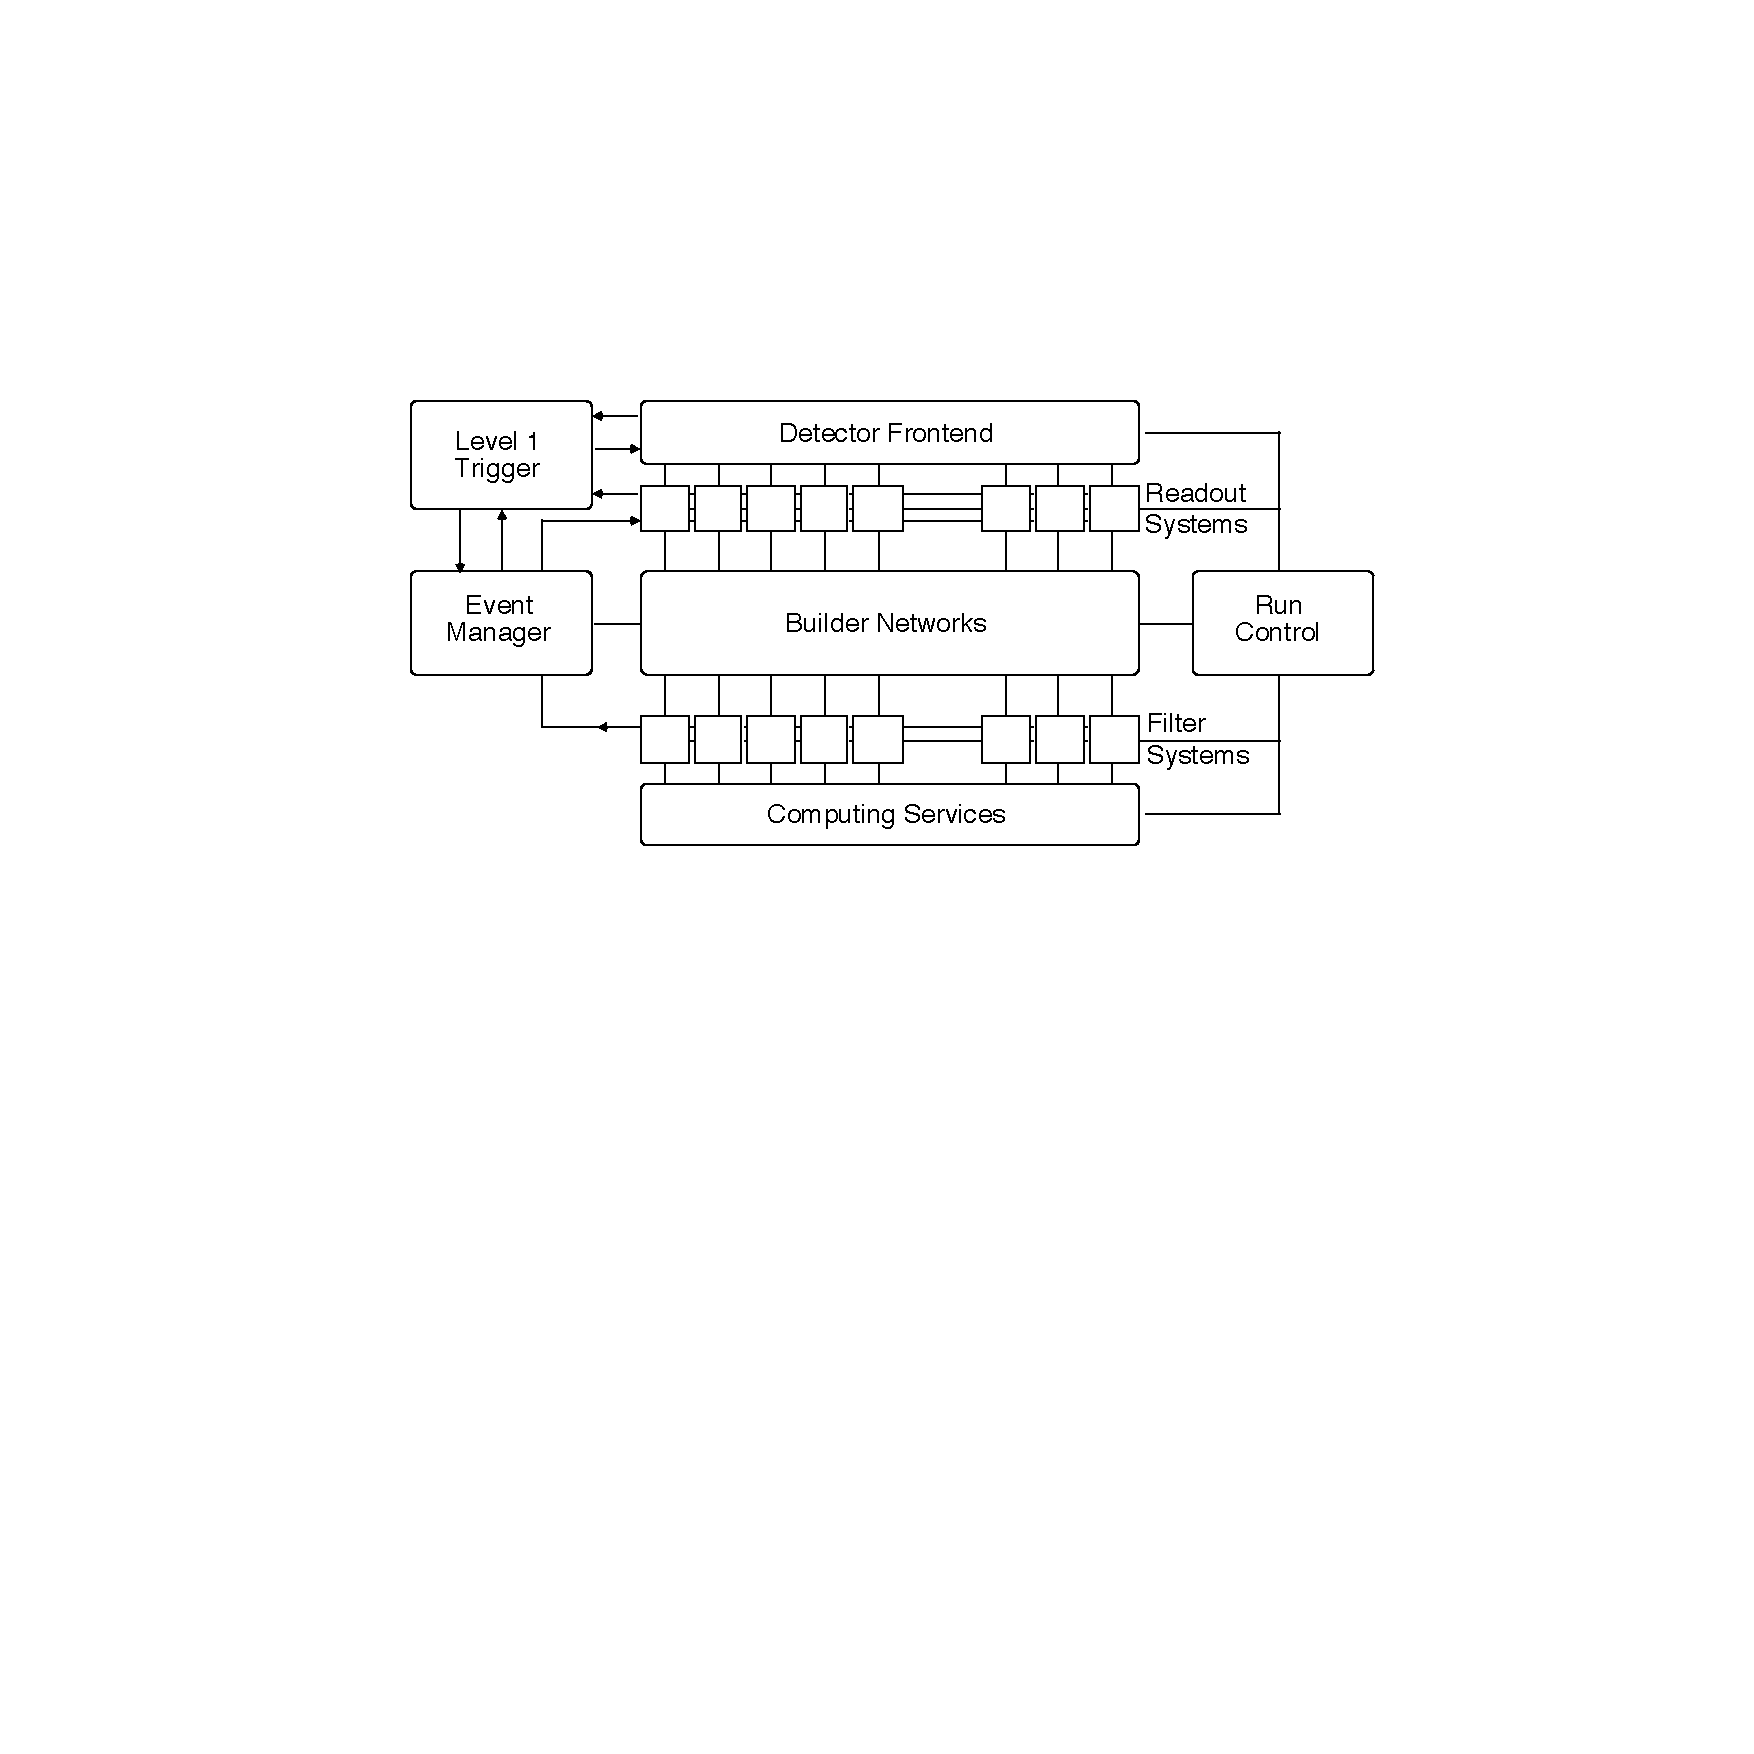
\includegraphics[width=0.9\textwidth]{cms/img/trigger}
\caption{CMS Trigger and Data Acquisition System.}
\label{fig:trigger}
\end{figure}
At the first level all information about the event is preserved.
The first level decision is made, with negligible dead-time, on a
subset of the total information available for the events. Since signal propagation delays are included in
this pipeline time, the L$1$ trigger calculations must be done in
many cases in less than $1 \, \mathrm{\mu s}$. If the first level trigger generates
an accept, the event data are moved or assigned to a buffer for
readout and processing by the High Level Triggers.



The L$1$ trigger involves the calorimetry and muon systems as well
as some correlation of information from these systems. The L$1$
decision is based on the presence of local objects such as photons,
electrons, muons, and jets, using information from calorimeters,
and muon systems in a given element of $\eta$-$\phi$ space. It also employs
global sums of $E_T$ and missing $E_T$. Each of these items is tested
against several $p_T$ or $E_T$ thresholds.


\subsection{High Level Trigger}

The CMS Level-$1$ Trigger System is required to reduce the input
interaction rate of $1 \,$GHz to a filtered event rate of $75 \,$kHz. 
To match the capabilities of the mass storage and offline computing systems, the final output of the
experiment should not exceed $100$ events per second.


The High Level Triggers have access to all the information used in
L$1$ since this is stored locally in the L$1$ trigger crates. Consequently,
High Level Triggers can make further combinations and other topological
calculations on the digital list of objects transmitted from L$1$.
Eventually, the High Level Triggers use the full event data for the decision
to keep an event.
\end{comment}


